\documentclass[a4paper, 11pt]{article}

\usepackage{graphicx}
\usepackage{geometry}
\usepackage[export]{adjustbox}

\geometry{a4paper, margin=1.2in}

\providecommand{\tightlist}{%
    \setlength{\itemsep}{0pt}
    \setlength{\parskip}{0pt}
}

\begin{document}

\section{Gebruikershandleiding SAP-omgeving}

Vereisten:

\begin{itemize}
\tightlist
\item
  SAP GUI for Java / SAP Gui for Windows
\item
  Virtualbox versie: v5.2.8 of later
\item
  sap-omgeving.ova bestand
\end{itemize}

\subsection{Installatie}

\begin{enumerate}
\tightlist
\item
  Dubbelklik op de sap-omgeving.ova file. Dit opent automatisch
  virtualbox.
\item
  Klik op \texttt{Import} om de virtuele machine te importeren.
  \begin{center}
      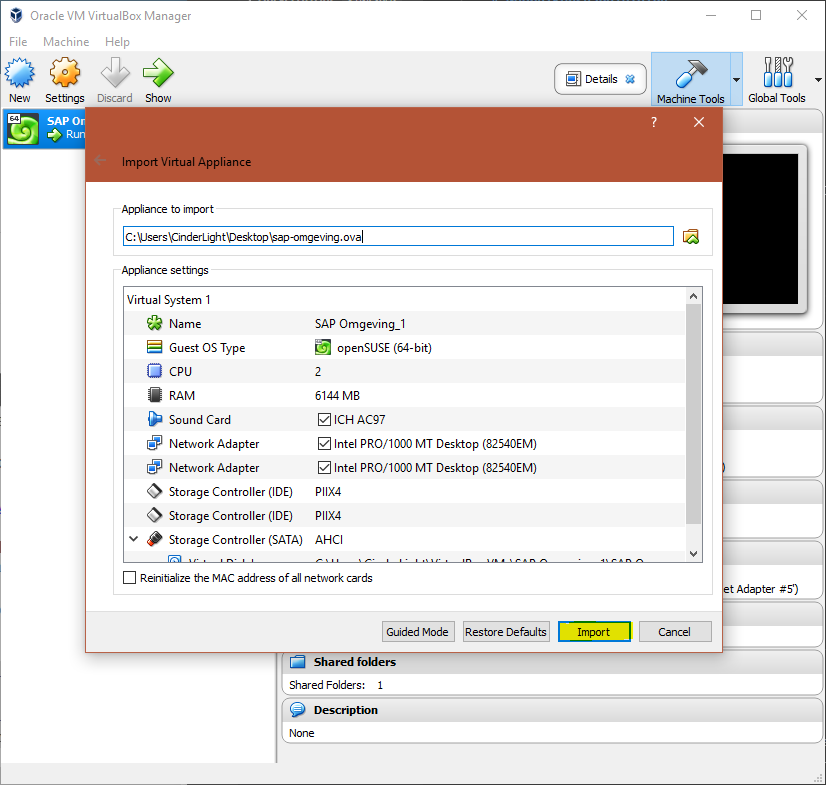
\includegraphics[scale=0.7,center]{img/import.png}
  \end{center}
\end{enumerate}

\begin{enumerate}
\setcounter{enumi}{2}
\tightlist
\item
  Wacht tot de virtuele machine geïmporteerd is.
\item
  Start de machine met de \texttt{Headless\ start} optie. Wacht een tweetal minuten alvorens te connecteren, zodat de server volledig kan opstarten.
  \begin{center}
    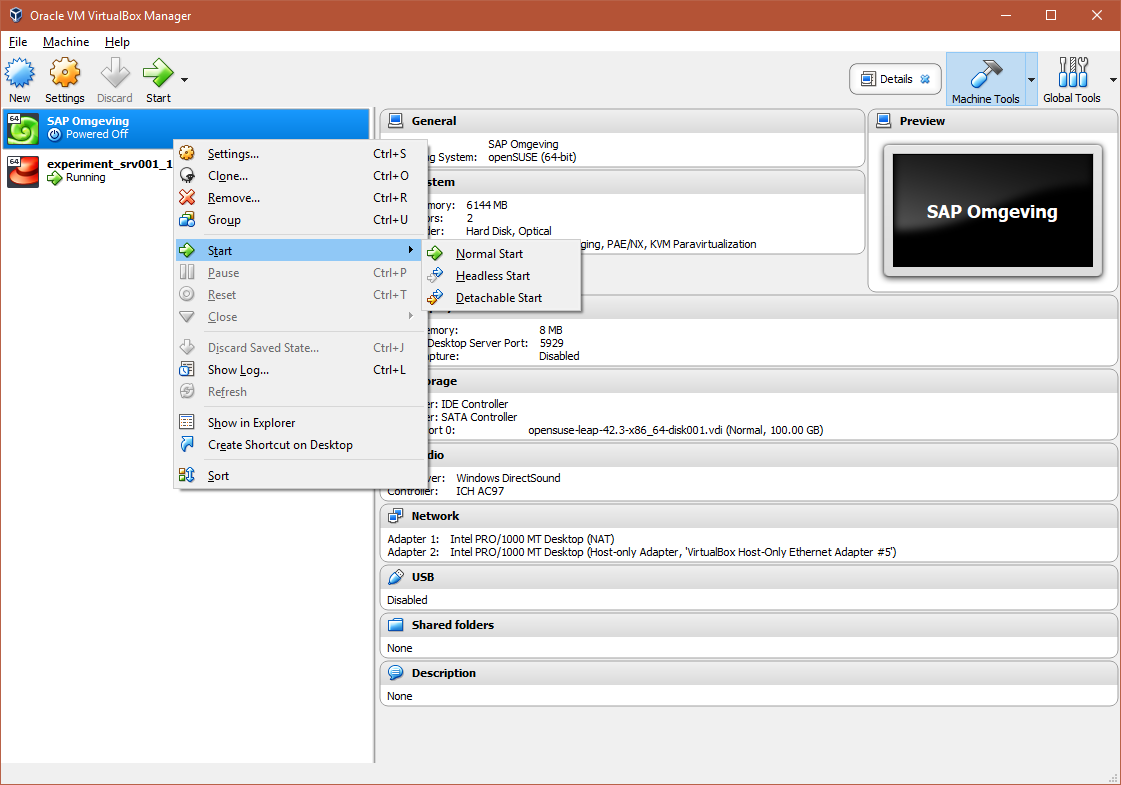
\includegraphics[scale=0.55,center]{img/start.png}
  \end{center}
\end{enumerate}

\subsection{Connecteren met SAP GUI for Java}

\begin{enumerate}
\tightlist
\item
  Open de SAP GUI for Java.
\item
  Klik op \texttt{New\ Connection} onder het menu \texttt{File}.
  \begin{center}
    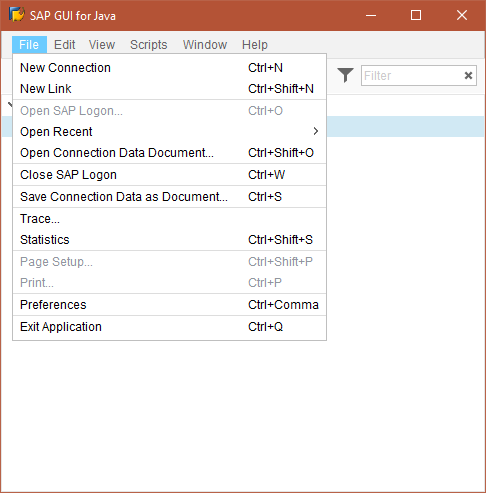
\includegraphics[scale=0.7,center]{img/file.png}
  \end{center}
\end{enumerate}

\begin{enumerate}
\setcounter{enumi}{2}
\tightlist
\item
  Vul de vereiste velden in volgens onderstaande foto.
\begin{center}
    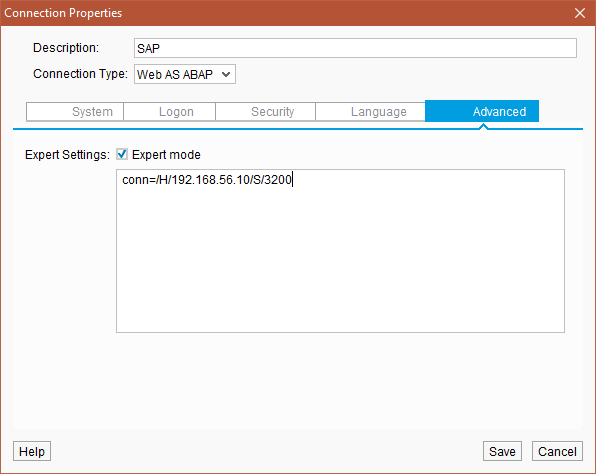
\includegraphics[scale=0.9,center]{img/connectie.png}
\end{center}
\end{enumerate}

\begin{enumerate}
\def\labelenumi{\arabic{enumi}.}
\setcounter{enumi}{3}
\tightlist
\item
  Druk vervolgens op \texttt{Save} en je server wordt toegevoegd aan de
  lijst in de SAP-client.
\item
  Ten slotte selecteer je de server en maak je verbinding door op \texttt{Connect} te drukken.
 \begin{center}
    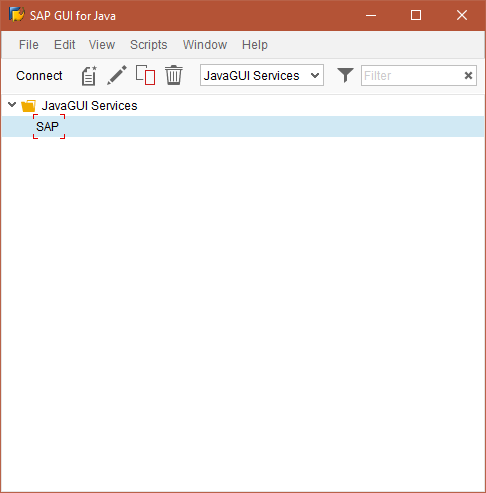
\includegraphics[scale=0.76,center]{img/sap.png}
\end{center}
\end{enumerate}

\subsection{Connecteren met SAP GUI for Windows}

\begin{enumerate}
\tightlist
\item
  Open de SAP GUI for Windows.
\item
  Klik op \texttt{New} voor een nieuwe connectie te maken.
\begin{center}
    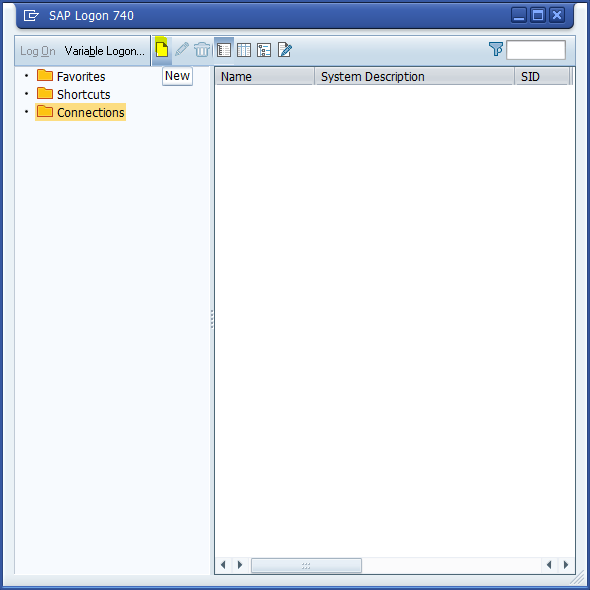
\includegraphics[scale=0.60,center]{img/windows.png}
\end{center}
\end{enumerate}

\begin{enumerate}
\setcounter{enumi}{2}
\tightlist
\item
  Op het volgende venster klik je op \texttt{Next}.
\item
  Vul de vereiste velden in volgens onderstaande foto.
\begin{center}
    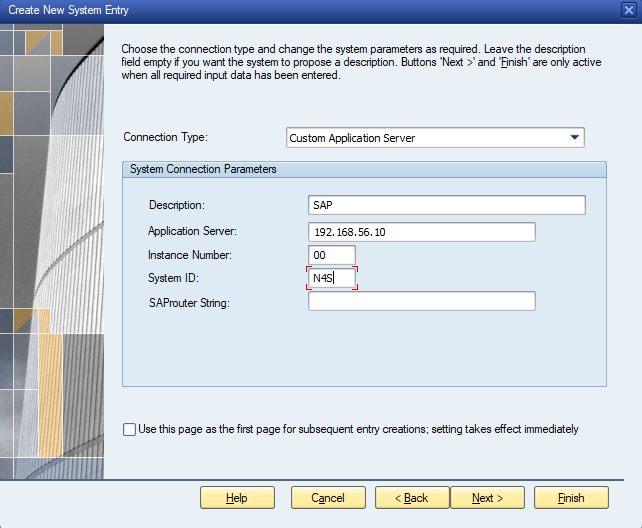
\includegraphics[scale=0.68,center]{img/server.png}
\end{center}
\end{enumerate}

\begin{enumerate}
\setcounter{enumi}{4}
\tightlist
\item
  Druk vervolgens nog twee maal op \texttt{Next} en nog een keer op
  \texttt{Finish}.
\item
  Ten slotte maak je verbinding met de server door te dubbelklikken op
  \texttt{SAP}.
\end{enumerate}

\subsection{Server aflsuiten}

\begin{enumerate}
 \item 
  Alvorens je pc af te sluiten, moet je eerst de server uitzetten. Hiervoor druk je op `ACPI Shutdown`.
\end{enumerate}
\begin{center}
    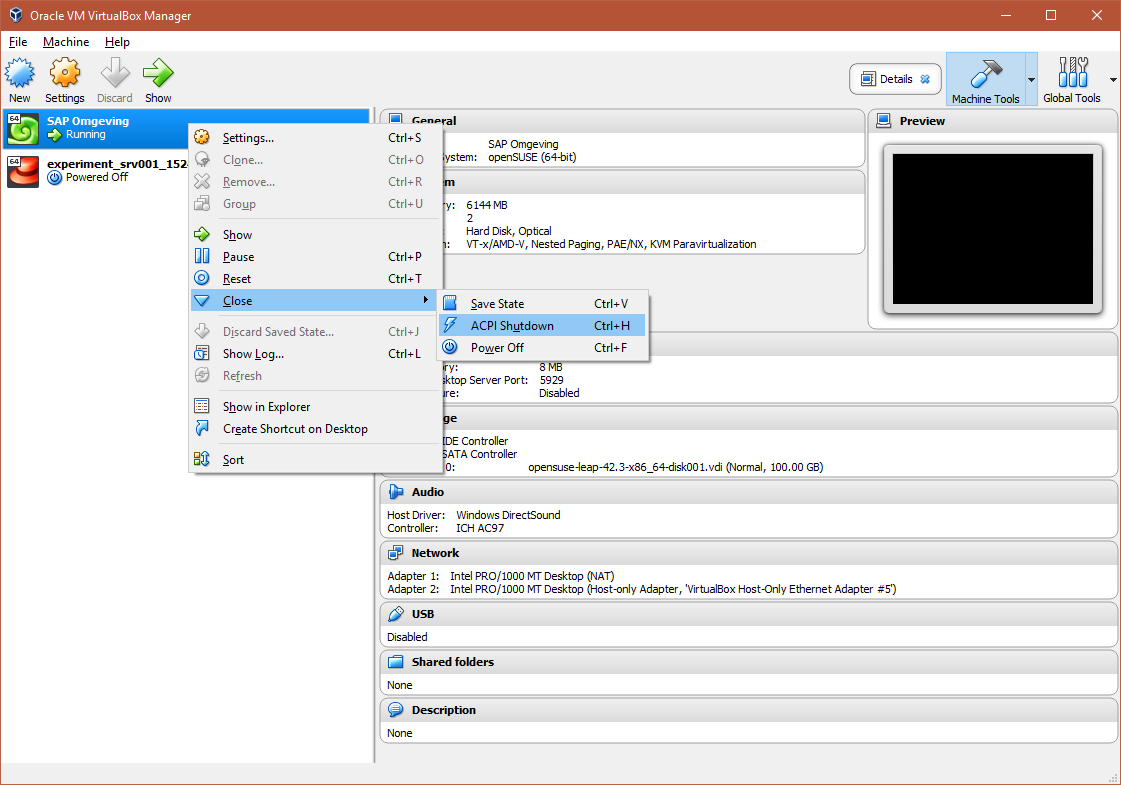
\includegraphics[scale=0.68,center]{img/shutdown.png}
\end{center}

\end{document}
